\documentclass[11pt,a4paper]{article}

\usepackage[utf8]{inputenc}
\usepackage[T1]{fontenc}
\usepackage[french]{babel}

\usepackage[default]{sourcesanspro}
\usepackage{fontawesome5}
\usepackage{microtype}
\usepackage{setspace}
\linespread{1.15}

\usepackage[top=2.2cm, bottom=2.2cm, left=2.2cm, right=2.2cm]{geometry}
\usepackage{indentfirst}
\setlength{\parindent}{0.5cm}
\setlength{\parskip}{0.3em}

\usepackage{xcolor}
\definecolor{main}{HTML}{1F4E79}
\definecolor{accent}{HTML}{2E86AB}
\definecolor{light}{HTML}{F5F7FA}

\usepackage{titlesec}

\titleformat{\section}
  {\Large\bfseries\color{main}}
  {}
  {0em}
  {}
  [\vspace{0.3em}\titlerule]

\titleformat{\subsection}
  {\normalsize\bfseries\color{accent}}
  {}
  {0em}
  {}

\titlespacing*{\section}{0pt}{2.5ex}{1.2ex}
\titlespacing*{\subsection}{0pt}{2ex}{0.8ex}

\usepackage{booktabs}
\usepackage{array}
\usepackage{multirow}
\renewcommand{\arraystretch}{1.25}

\usepackage{graphicx}
\usepackage{float}
\usepackage{caption}
\usepackage{subcaption}

\captionsetup{
  font=small,
  labelfont=bf
}

\usepackage{amsmath}
\usepackage{amssymb}

\usepackage[colorlinks=true,
linkcolor=main,
urlcolor=accent]{hyperref}

\usepackage[most]{tcolorbox}

\tcbset{
  colback=light,
  colframe=main,
  arc=8pt,
  boxrule=0.8pt,
  left=10pt,
  right=10pt,
  top=6pt,
  bottom=6pt,
  drop fuzzy shadow
}

\usepackage{enumitem}
\setlist[itemize]{noitemsep, topsep=4pt}

\usepackage{fancyhdr}
\pagestyle{fancy}
\fancyhf{}
\fancyhead[L]{\small\textcolor{gray}{Projet Statistique}}
\fancyhead[R]{\small\textcolor{gray}{2025--2026}}
\fancyfoot[C]{\thepage}
\renewcommand{\headrulewidth}{0pt}

% ─────────────────────────────────────────────────────
\begin{document}

% Page de titre
\begin{titlepage}
\centering

\vspace*{2cm}

{\Huge\bfseries\color{main}
Salaires au baseball
}

\vspace{0.4cm}

{\Large La performance paie-t-elle ?}

\vspace{1cm}

\rule{0.4\linewidth}{1pt}

\vspace{1.5cm}

{\large
Analyse statistique des joueurs de MLB\\
Saison 1992 -- 337 joueurs
}

\vspace{2cm}

{\large
\textcolor{main}{\faUniversity} \textsc{Université Paris Cité} \\
\vspace{0.2cm}
\normalsize{\faGraduationCap\ Licence 3 | Outils pour la Data Science}
}

\vspace{1.5cm}

{\normalsize
\faUser\ AIT MESSAOUD Mohamed Said\\
\faUser\ TAKENNE MEKEM Simeon\\
\faUser\ ZEROUALI Amine
}

\vspace{0.8cm}

\faChalkboardTeacher\ Encadrants : J. Collet \& R. Mozet\\
\vspace{0.3cm}
\faGithub\ \href{https://github.com/Amine-Zerouali/mlb-baseball-salary-analysis}{\color{accent}Code source et données (GitHub)}

\vfill

{\small Février -- Mai 2026}

\end{titlepage}

% Table des matières 
\enlargethispage{2\baselineskip}
\tableofcontents
\newpage

\titlespacing*{\section}{0pt}{2.5ex}{1.5ex}
\titlespacing*{\subsection}{0pt}{2ex}{1ex}

% =============================================================================
\renewcommand{\abstractname}{Synthèse}
\section*{Synthèse}
\addcontentsline{toc}{section}{Synthèse}

\textit{Les analyses statistiques menées dans ce rapport mettent en évidence quatre résultats majeurs concernant la rémunération des joueurs de la MLB :}

\begin{itemize}
    \item \textbf{Le volume prime sur la qualité pure :} Le nombre de coups sûrs (\textit{Hits}) et de points produits (\textit{RBI}) explique près de la moitié de la variance des salaires, loin devant la moyenne au bâton.\vspace{0.3cm}
    \item \textbf{Le pouvoir de marché est déterminant :} À statistiques égales, un joueur éligible à l'agence libre perçoit un salaire jusqu'à 4 fois supérieur à celui d'un joueur sous contrat restreint.\vspace{0.3cm}
    \item \textbf{L'arbitrage comme levier d'accélération :} C'est pour les joueurs éligibles à l'arbitrage que la performance marginale (un coup sûr supplémentaire) est la mieux valorisée financièrement ($+0.68\%$ par hit).\vspace{0.3cm}
    \item \textbf{Identification de 3 profils distincts :} L'ACP et la classification mettent en évidence trois typologies claires (Titulaires, Remplaçants, Profils atypiques) corroborant parfaitement la hiérarchie salariale.
\end{itemize}

% =============================================================================
\section*{Introduction}
\addcontentsline{toc}{section}{Introduction}

Le baseball constitue un terrain d'étude privilégié pour l'économiste du travail : les
performances individuelles des joueurs sont mesurées de façon précise et standardisée,
ce qui permet d'évaluer quantitativement la contribution de chaque employé à la
production collective. Ce projet s'inscrit dans cette tradition en cherchant à répondre
à une question centrale : \textbf{les salaires des joueurs de baseball sont-ils déterminés
par leur performance sportive ?}\vspace{0.3cm}

Nous disposons pour cela d'un jeu de données regroupant 337 joueurs de la
\textit{Major League Baseball} (MLB) ayant participé à au moins un match lors des
saisons 1991 et 1992 (les lanceurs sont exclus). Pour chaque joueur, nous observons
son salaire 1992 (en milliers de dollars), ses statistiques offensives de la saison 1991,
ainsi que son statut contractuel (éligibilité à l'agence libre, à l'arbitrage).\vspace{0.3cm}

La démarche suivie est progressive. Après une analyse descriptive du jeu de données
(partie 1) et des analyses univariées (partie 2), nous étudions les liaisons entre le
salaire et les variables explicatives (partie 3). Nous construisons ensuite des modèles
de régression simple (partie 4) puis multiple (partie 5), avant de clore l'étude par
une analyse en composantes principales (ACP) couplée à une classification ascendante
hiérarchique (CAH) réalisée sous R (partie 6).

% =============================================================================
\section{Analyse descriptive du jeu de données}

\subsection{Structure du jeu de données}

Le jeu de données comporte \textbf{337 observations} et \textbf{18 variables}. On
distingue :
\begin{itemize}
  \item 1 variable à expliquer : \texttt{Salary}, le salaire 1992 en milliers de dollars ;\vspace{0.3cm}
  \item 12 variables de performance continue issues de la saison 1991 :
        moyenne au bâton (\texttt{Batting\_avg}), pourcentage d'atteinte de la base
        (\texttt{OBP}), nombre de points (\texttt{Runs}), de coups sûrs (\texttt{Hits}),
        de doubles, de triples, de home runs (\texttt{HR}), de points produits
        (\texttt{RBI}), de buts sur balles (\texttt{Walks}), de retraits au bâton
        (\texttt{Strike\_outs}), de buts volés (\texttt{Stolen\_Bases}) et d'erreurs ;\vspace{0.3cm}
  \item 4 variables binaires de statut contractuel : éligibilité à l'agence libre
        (\texttt{Free\_agency\_elig}), statut d'agent libre en 1991/92
        (\texttt{Free\_agent\_91\_92}), éligibilité à l'arbitrage
        (\texttt{Arbitration\_elig}), et arbitrage en 1991/92
        (\texttt{Arbitration\_91\_92}).
\end{itemize}

\noindent\textbf{Valeurs manquantes.} Le tableau \ref{tab:means} indique l'absence
totale de valeurs manquantes pour l'ensemble des 14 variables continues (N = 337
pour chacune), ce qui simplifie l'analyse.

\subsection{Statistiques descriptives}

\begin{table}[H]
\centering
\caption{Statistiques descriptives des variables continues (PROC MEANS)}
\label{tab:means}
\small
\begin{tabular}{lrrrrrr}
\toprule
\textbf{Variable} & \textbf{N} & \textbf{Moyenne} & \textbf{Médiane}
  & \textbf{Éc.-type} & \textbf{Min} & \textbf{Max} \\
\midrule
Salary (k\$)    & 337 & 1\,248.53 & 740.00  & 1\,240.01 & 109    & 6\,100  \\
LogSalary       & 337 & 6.535     & 6.607   & 1.177     & 4.691  & 8.716   \\
Batting\_avg    & 337 & 0.258     & 0.260   & 0.040     & 0.063  & 0.457   \\
OBP             & 337 & 0.324     & 0.323   & 0.047     & 0.063  & 0.486   \\
Runs            & 337 & 46.70     & 41.00   & 29.02     & 0      & 133     \\
Hits            & 337 & 92.83     & 91.00   & 51.90     & 1      & 216     \\
Doubles         & 337 & 16.67     & 15.00   & 10.45     & 0      & 49      \\
Triples         & 337 & 2.34      & 2.00    & 2.54      & 0      & 15      \\
HR              & 337 & 9.10      & 6.00    & 9.29      & 0      & 44      \\
RBI             & 337 & 44.02     & 39.00   & 29.56     & 0      & 133     \\
Walks           & 337 & 35.02     & 30.00   & 24.84     & 0      & 138     \\
Strike\_outs    & 337 & 56.71     & 49.00   & 33.83     & 1      & 175     \\
Stolen\_Bases   & 337 & 8.25      & 4.00    & 11.66     & 0      & 76      \\
Errors          & 337 & 6.77      & 5.00    & 5.93      & 0      & 31      \\
\bottomrule
\end{tabular}
\end{table}

Plusieurs observations ressortent de ce tableau. Le salaire moyen (1\,249 k\$) est
très supérieur à la médiane (740 k\$), signe d'une forte asymétrie droite : quelques
stars tirent la moyenne vers le haut. L'écart-type (1\,240 k\$) est du même ordre
que la moyenne, traduisant une dispersion considérable. Les variables de performance
présentent également une forte hétérogénéité : le nombre de coups sûrs varie de 1 à
216, les home runs de 0 à 44.

\subsection{Répartition des variables de statut contractuel}

\begin{table}[H]
\centering
\caption{Répartition des variables de statut contractuel (PROC FREQ)}
\label{tab:freq}
\begin{tabular}{lrrrr}
\toprule
\multirow{2}{*}{\textbf{Variable}} & \multicolumn{2}{c}{\textbf{Modalité 0}} & \multicolumn{2}{c}{\textbf{Modalité 1}} \\
\cmidrule(lr){2-3} \cmidrule(lr){4-5}
 & \textbf{N} & \textbf{\%} & \textbf{N} & \textbf{\%} \\
\midrule
Free\_agency\_elig    & 203 & 60.2\% & 134 & 39.8\% \\
Free\_agent\_91\_92   & 298 & 88.4\% & 39  & 11.6\% \\
Arbitration\_elig     & 272 & 80.7\% & 65  & 19.3\% \\
Arbitration\_91\_92   & 327 & 97.0\% & 10  & 3.0\%  \\
\bottomrule
\end{tabular}
\end{table}

Environ 40\,\% des joueurs sont éligibles à l'agence libre, ce qui leur confère la
liberté de négocier avec d'autres équipes. Seuls 11.6\,\% ont effectivement exercé ce
statut en 1991/92. L'arbitrage reste peu fréquent (moins de 20\,\% d'éligibles, moins
de 3\,\% l'ayant pratiqué). On notera que les deux statuts sont mutuellement exclusifs
dans les données : aucun joueur non-éligible à l'agence libre ne figure parmi les
agents libres effectifs.

% =============================================================================
\section{Analyses univariées}

\subsection{Distribution du salaire brut}

Le salaire brut présente une distribution fortement asymétrique à droite (Skewness $= 1.16$, Kurtosis $= 0.67$). Le test de Shapiro-Wilk rejette très nettement l'hypothèse de normalité ($W = 0.843$, $p < 0.0001$). L'histogramme (figure~\ref{fig:hist_salary}) confirme visuellement cette asymétrie : une grande concentration de joueurs dans les tranches basses (moins de $1\,000$~k\$) et une longue queue à droite avec quelques salaires dépassant $5\,000$~k\$. Le minimum du salaire ($109$~k\$, plancher syndical de l'époque) est atteint par plusieurs joueurs, ce qui crée un pic artificiel en bas de la distribution.

\begin{figure}[H]
  \centering
  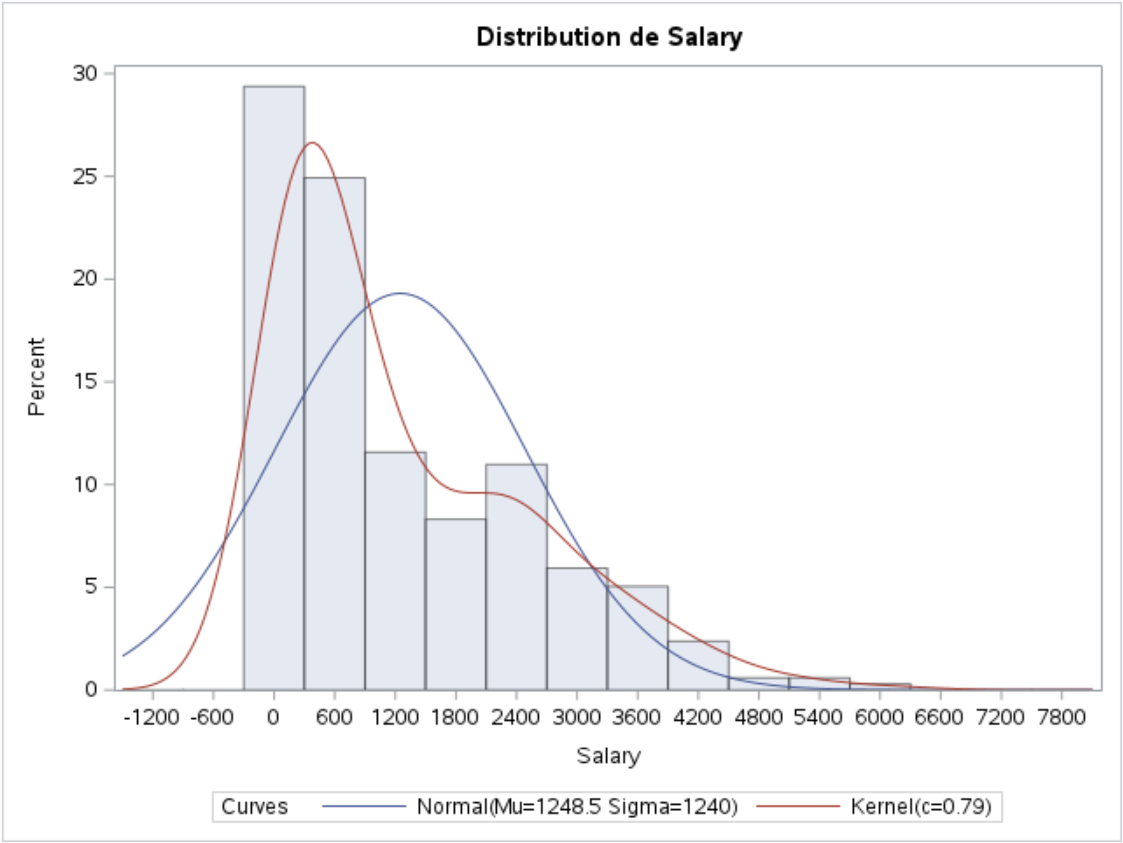
\includegraphics[width=0.65\linewidth]{Image/fig_hist_salary.png}
  \caption{Distribution du salaire brut (histogramme et courbe normale ajustée)}
  \label{fig:hist_salary}
\end{figure}

\subsection{Transformation logarithmique et normalité}

Afin de pallier l'asymétrie du salaire, nous appliquons une transformation
logarithmique : $\texttt{LogSalary} = \ln(\texttt{Salary})$. Cette transformation, classique pour des variables de revenus strictement positives et très étalées, produit une distribution nettement plus symétrique (Skewness $= -0.07$, quasi nulle).\vspace{0.3cm}

Cependant, les tests formels de normalité restent significatifs au seuil de 5\,\% même après transformation (Shapiro-Wilk : $W = 0.934$, $p < 0.0001$ ; Kolmogorov-Smirnov : $D = 0.102$, $p < 0.01$). Le graphique Q-Q (figure~\ref{fig:qq_logsalary}) révèle que l'écart à la normalité provient essentiellement des queues : les très petits salaires (plancher syndical) forment un palier en bas, et quelques super-stars créent une légère déviation en haut. Pour la modélisation par régression linéaire, la log-transformation reste justifiée car elle améliore nettement l’ajustement du modèle et rend les résidus plus homogènes.

\begin{figure}[H]
  \centering
  \begin{subfigure}[b]{0.48\linewidth}
    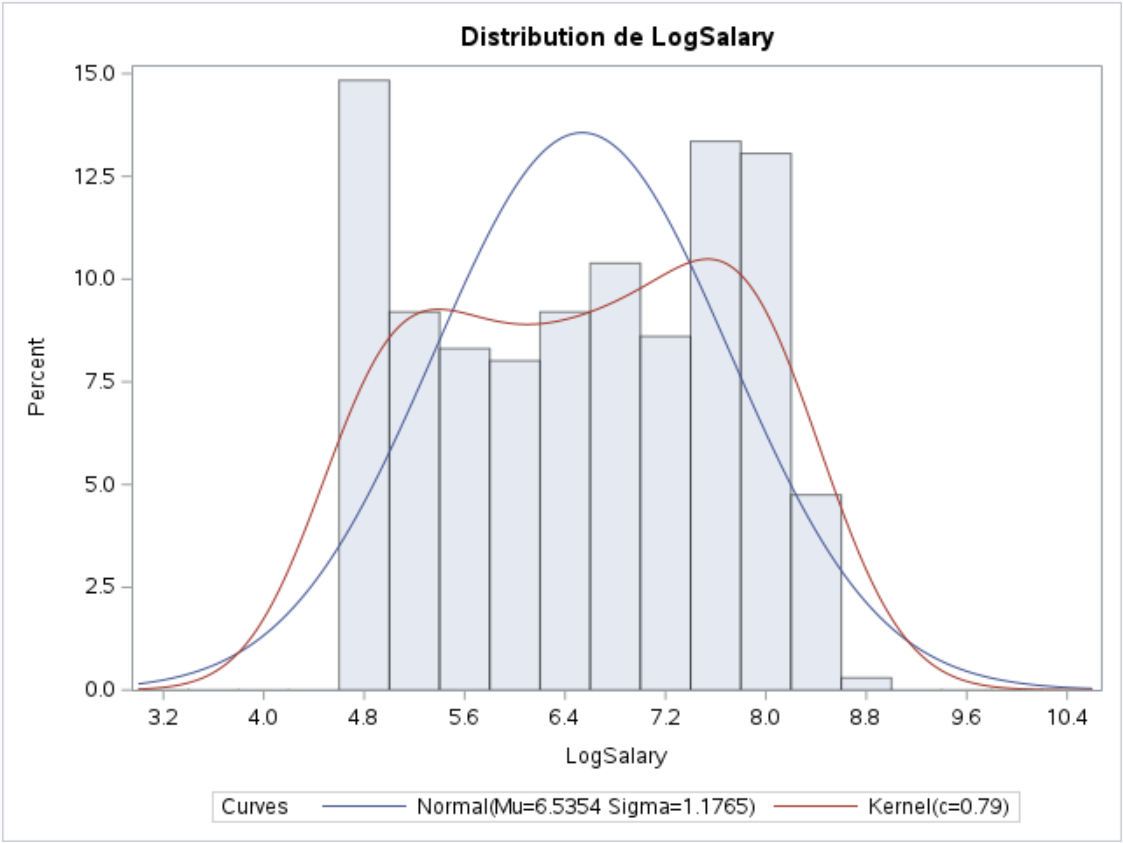
\includegraphics[width=\linewidth]{Image/fig_hist_logsalary.png}
    \caption{Histogramme de LogSalary}
  \end{subfigure}
  \hfill
  \begin{subfigure}[b]{0.48\linewidth}
    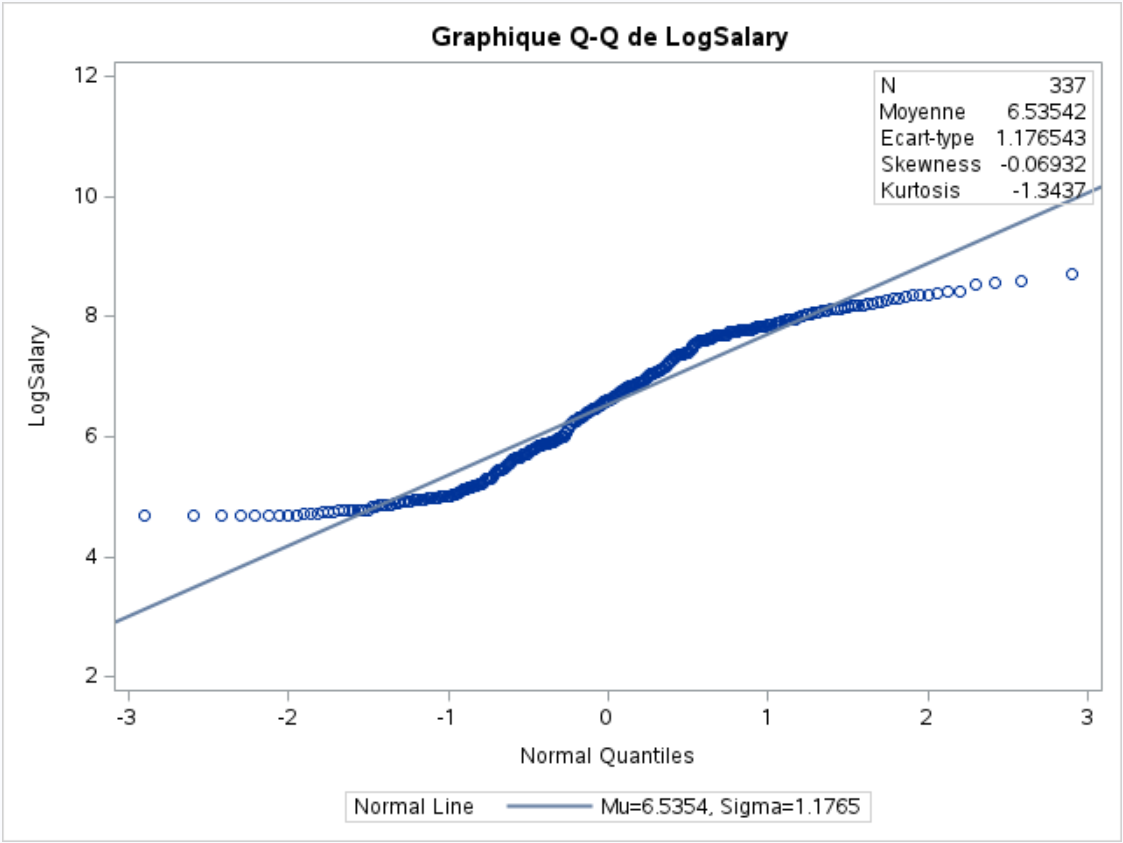
\includegraphics[width=\linewidth]{Image/fig_qq_logsalary.png}
    \caption{Graphique Q-Q de LogSalary}
  \end{subfigure}
  \caption{Distribution du log-salaire}
  \label{fig:qq_logsalary}
\end{figure}

\noindent\textbf{Variable à expliquer retenue.} Pour toute la suite, nous modélisons
\texttt{LogSalary} plutôt que \texttt{Salary}.

% =============================================================================
\section{Liaisons avec le salaire}

\subsection{Corrélations linéaires}

Le tableau~\ref{tab:corr} présente les coefficients de corrélation de Pearson entre
\texttt{LogSalary} et chacune des 16 variables explicatives. Toutes les variables de
performance sont significativement corrélées au seuil de 1\,\% (sauf \texttt{Arbitration\_91\_92}
qui atteint $p = 0.054$).

\begin{table}[H]
\centering
\caption{Corrélations de Pearson avec LogSalary (PROC CORR, $N = 337$)}
\label{tab:corr}
\small
\begin{tabular}{lrrl}
\toprule
\textbf{Variable} & \textbf{$r$} & \textbf{$p$-value} & \textbf{Interprétation} \\
\midrule
Hits              & 0.668 & $<0.0001$ & Très forte liaison positive \\
Runs              & 0.647 & $<0.0001$ & Très forte liaison positive \\
RBI               & 0.652 & $<0.0001$ & Très forte liaison positive \\
Doubles           & 0.599 & $<0.0001$ & Forte liaison positive \\
Walks             & 0.572 & $<0.0001$ & Forte liaison positive \\
HR                & 0.531 & $<0.0001$ & Liaison positive modérée \\
Free\_agency\_elig & 0.602 & $<0.0001$ & Forte liaison (statut) \\
Strike\_outs      & 0.414 & $<0.0001$ & Liaison positive modérée \\
OBP               & 0.306 & $<0.0001$ & Liaison positive faible \\
Arbitration\_elig & 0.251 & $<0.0001$ & Liaison positive faible \\
Triples           & 0.274 & $<0.0001$ & Liaison positive faible \\
Batting\_avg      & 0.266 & $<0.0001$ & Liaison positive faible \\
Stolen\_Bases     & 0.242 & $<0.0001$ & Liaison positive faible \\
Free\_agent\_91\_92 & 0.159 & $0.0034$  & Liaison faible \\
Errors            & 0.184 & $0.0007$  & Liaison positive faible \\
Arbitration\_91\_92 & 0.105 & $0.054$   & Non significatif \\
\bottomrule
\end{tabular}
\end{table}

Les variables \texttt{Hits} ($r = 0.668$), \texttt{RBI} ($r = 0.652$) et \texttt{Runs}
($r = 0.647$) présentent les corrélations les plus fortes avec le log-salaire. Le statut
de free agency (\texttt{Free\_agency\_elig}, $r = 0.602$) est aussi fortement lié au
salaire : les joueurs libres de négocier avec d'autres équipes sont mieux rémunérés.
À l'inverse, la moyenne au bâton (\texttt{Batting\_avg}, $r = 0.266$) et l'OBP
($r = 0.306$), malgré leur pertinence sportive, ont un pouvoir prédictif limité sur le
salaire, ce qui suggère que la quantité de jeu (volume) prime sur la qualité pure.

\subsection{Indépendance entre variables de statut contractuel}

Avant d'introduire les variables de statut dans un modèle de régression, nous
vérifions leur indépendance deux à deux par des tests du Chi² (PROC FREQ,
option \texttt{/CHISQ}). Les résultats sont présentés dans le tableau~\ref{tab:chi2}.

\begin{table}[H]
\centering
\caption{Tests d'indépendance du Chi² entre variables de statut contractuel}
\label{tab:chi2}
\small
\begin{tabular}{llrrr}
\toprule
\textbf{Variable 1} & \textbf{Variable 2} & \textbf{$\chi^2$} & \textbf{$p$-value} & \textbf{Conclusion} \\
\midrule
Free\_agency\_elig   & Arbitration\_elig    & 53.16 & $<0.0001$ & Dépendantes \\
Free\_agency\_elig   & Free\_agent\_91\_92  & 66.81 & $<0.0001$ & Dépendantes \\
Free\_agency\_elig   & Arbitration\_91\_92  & 6.80  & $0.009$   & Dépendantes \\
Arbitration\_elig    & Free\_agent\_91\_92  & 10.54 & $0.001$   & Dépendantes \\
Arbitration\_elig    & Arbitration\_91\_92  & 43.13 & $<0.0001$ & Dépendantes \\
\textbf{Free\_agent\_91\_92} & \textbf{Arbitration\_91\_92}
  & \textbf{1.35} & \textbf{0.245} & \textbf{Indépendantes} \\
\bottomrule
\end{tabular}
\end{table}

Cinq des six paires sont significativement dépendantes. Deux dépendances sont
\textbf{structurelles} : on ne peut être agent libre sans y être éligible, et
de même pour l'arbitrage. Plus intéressante, la dépendance entre
\texttt{Free\_agency\_elig} et \texttt{Arbitration\_elig} ($\chi^2 = 53.16$)
révèle que ces deux statuts sont \textbf{mutuellement exclusifs} : aucun joueur
n'est à la fois éligible à l'agence libre et à l'arbitrage (cellule $= 0$ dans le
tableau croisé).\vspace{0.3cm}

Cette exclusivité mutuelle nous amène à construire une variable synthétique
\texttt{Statut} à trois modalités, fusionnant les deux variables d'éligibilité :
\begin{itemize}
  \item \texttt{0\_Aucun} : joueur sous contrat restreint (138 joueurs, 41.0\,\%) ;\vspace{0.3cm}
  \item \texttt{1\_Arbitrage} : éligible à l'arbitrage (65 joueurs, 19.3\,\%) ;\vspace{0.3cm}
  \item \texttt{2\_AgentLibre} : éligible à l'agence libre (134 joueurs, 39.8\,\%).
\end{itemize}

La seule paire \textbf{indépendante} est \texttt{Free\_agent\_91\_92}
$\times$ \texttt{Arbitration\_91\_92} ($\chi^2 = 1.35$, $p = 0.245$) :
ces deux procédures contractuelles sont mutuellement exclusives dans la pratique.
Cette variable \texttt{Statut} sera utilisée dans la régression multiple
(partie 5) en remplacement des deux variables d'éligibilité séparées.

\subsection{Effet du statut contractuel sur le salaire}

Nous réalisons deux tests de Student pour comparer les distributions de
\texttt{LogSalary} selon le statut contractuel.

\paragraph{Éligibilité à l'agence libre.}
Les joueurs éligibles à l'agence libre gagnent en moyenne
$e^{7.406} \approx 1\,644$~k\$ contre $e^{5.961} \approx 387$~k\$ pour les autres,
soit un rapport de \textbf{4,2}. Cette différence est hautement significative
($t = -13.79$, $p < 0.0001$). Les variances étant inégales (test de Levene :
$F = 1.54$, $p = 0.007$), on retient la correction de Satterthwaite, qui confirme le
résultat ($t = -14.41$, $p < 0.0001$).

\paragraph{Statut d'agent libre en 1991/92.}
Les joueurs ayant exercé leur droit d'agent libre en 1991/92 gagnent en moyenne
$e^{7.053} \approx 1\,151$~k\$ contre $e^{6.468} \approx 641$~k\$ ($t = -2.95$,
$p = 0.003$). Cette différence est significative mais plus modeste, et le graphe Q-Q
(figure~\ref{fig:ttest}) montre que le groupe « agent libre » présente une très bonne
adéquation à la loi normale.

\begin{figure}[H]
  \centering
  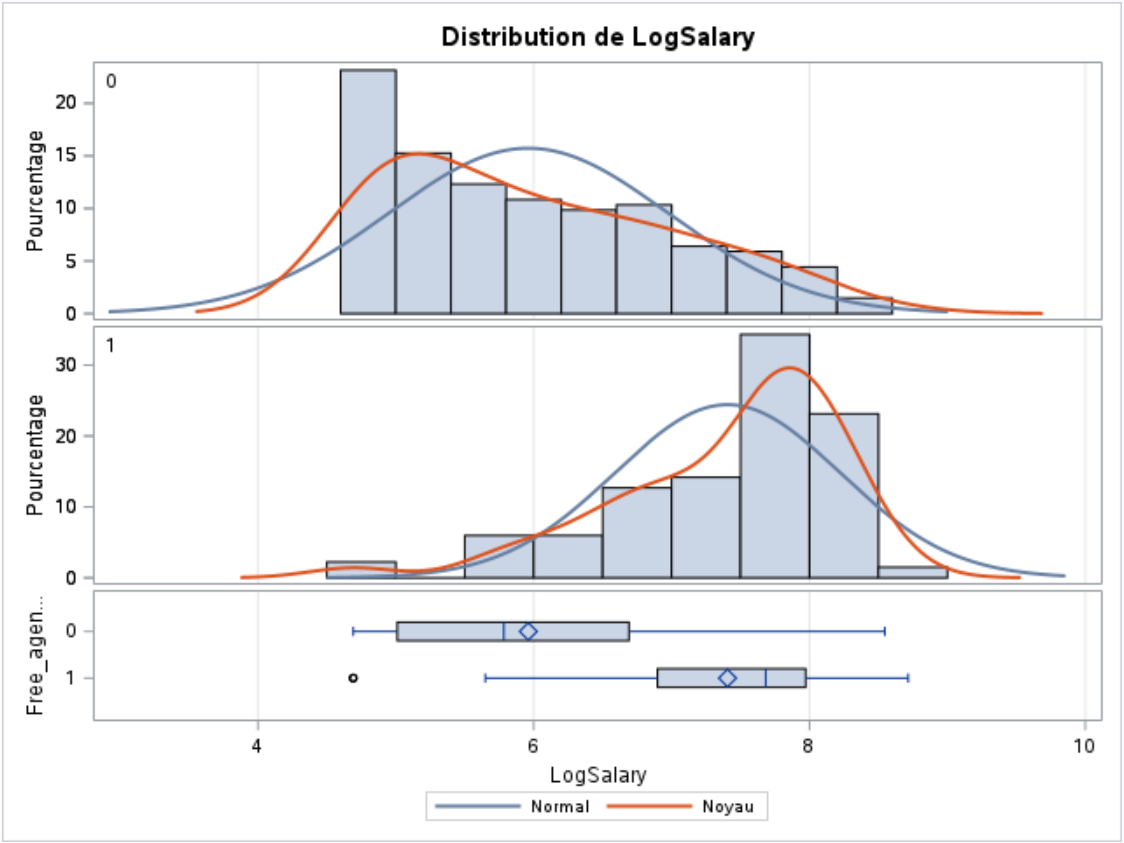
\includegraphics[width=0.75\linewidth]{Image/fig_ttest_freeagency.png}
  \caption{Distribution de LogSalary selon le statut de free agency (PROC TTEST)}
  \label{fig:ttest}
\end{figure}

Ces résultats illustrent l'importance de la liberté contractuelle dans la détermination
des salaires : au-delà de la performance sportive, le \textit{pouvoir de négociation}
du joueur joue un rôle déterminant.

% =============================================================================
\section{Régressions simples}

\subsection{Comparaison des quatre modèles}

Nous ajustons quatre modèles de régression simple de \texttt{LogSalary} sur les
variables de performance les plus corrélées. Les résultats sont résumés dans le
tableau~\ref{tab:reg_simples}.

\begin{table}[H]
\centering
\caption{Comparaison des régressions simples (PROC REG)}
\label{tab:reg_simples}
\begin{tabular}{lrrrl}
\toprule
\textbf{Modèle} & \textbf{$r$} & \textbf{$R^2$} & \textbf{$p$-value ($F$)} & \textbf{Signe} \\
\midrule
LogSalary $\sim$ Hits         & 0.668 & 0.446 & $<0.0001$ & $+$ \\
LogSalary $\sim$ RBI          & 0.652 & 0.425 & $<0.0001$ & $+$ \\
LogSalary $\sim$ Runs         & 0.647 & 0.419 & $<0.0001$ & $+$ \\
LogSalary $\sim$ HR           & 0.531 & 0.282 & $<0.0001$ & $+$ \\
LogSalary $\sim$ Batting\_avg & 0.266 & 0.071 & $<0.0001$ & $+$ \\
\bottomrule
\end{tabular}
\end{table}



La variable \textbf{Hits} est la meilleure variable explicative simple ($R^2 = 0.446$) :
elle explique près de 45\,\% de la variance du log-salaire. Ce résultat est cohérent
avec l'interprétation des auteurs du jeu de données, qui considèrent \texttt{Hits}
comme un proxy du temps de jeu effectif. En revanche, la moyenne au bâton
(\texttt{Batting\_avg}) est un mauvais prédicteur ($R^2 = 0.071$) : la qualité
intrinsèque du joueur est moins valorisée que sa présence sur le terrain.\footnote{Les $R^2$ sont calculés à partir des corrélations de Pearson ($R^2 = r^2$) et confirmés par PROC REG.}

\subsection{Analyse du modèle retenu : LogSalary $\sim$ Hits}

Le modèle estimé par PROC REG est (tous les paramètres sont significatifs à
$p < 0.0001$) :
\[
  \widehat{\texttt{LogSalary}} = 5.131 + 0.01513 \times \texttt{Hits}
  \qquad (R^2 = 0.446,\ \text{RMSE} = 0.877)
\]

\noindent Le coefficient $0.01513$ s'interprète ainsi : un coup sûr
supplémentaire est associé en moyenne à une hausse de
$e^{0.01513} - 1 \approx \textbf{1.52\,\%}$ du salaire. Sur une saison,
un joueur passant de 100 à 150 coups sûrs voit son salaire multiplié par
$e^{50 \times 0.01513} \approx 2.1$.

\paragraph{Diagnostics (figure~\ref{fig:diag_reg}).}
Le graphique des résidus en fonction des valeurs prédites montre une légère variation de la dispersion : les résidus sont plus étalés pour les petites valeurs prédites (joueurs peu actifs). C’est assez logique, car le modèle a du mal à différencier les contrats proches du minimum syndical. Le graphique Q-Q indique que les résidus suivent globalement une distribution normale au centre, avec quelques écarts aux extrémités (valeurs atypiques).

\begin{figure}[H]
  \centering
  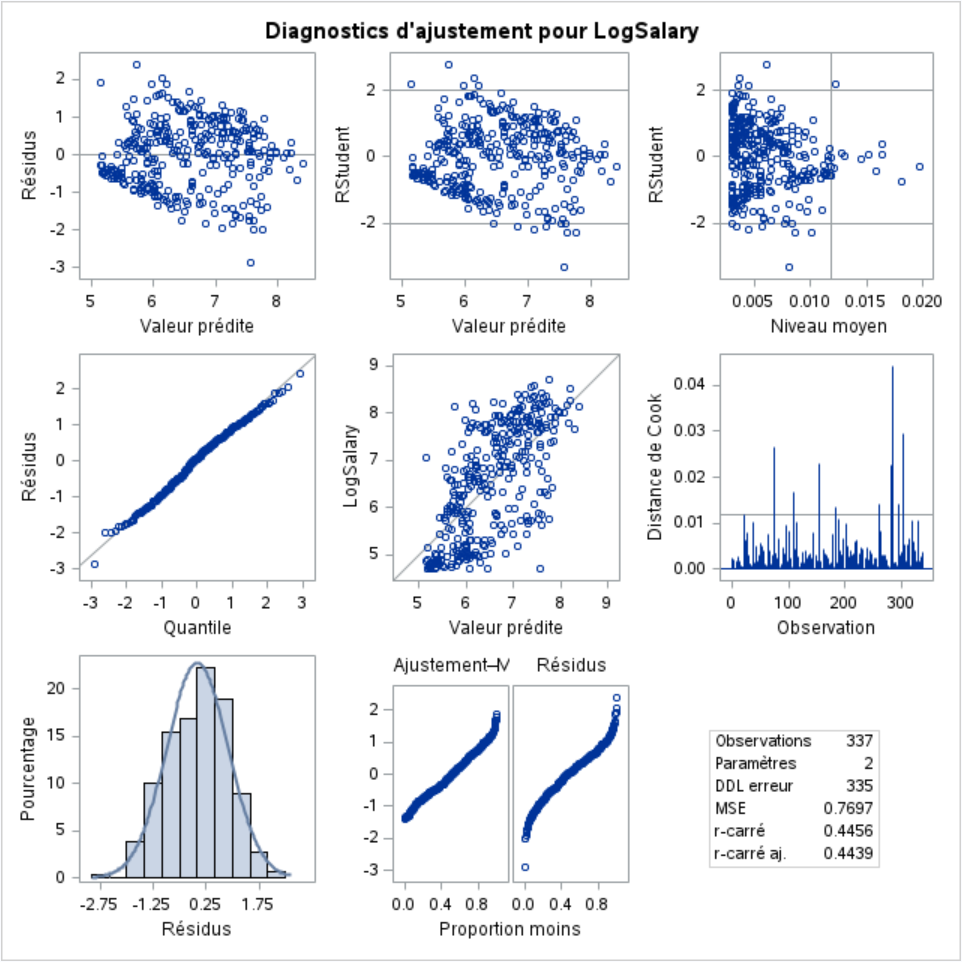
\includegraphics[width=0.70\linewidth]{Image/fig_diag_reg.png}
  \caption{Diagnostics d'ajustement du modèle LogSalary $\sim$ Hits (PROC REG)}
  \label{fig:diag_reg}
\end{figure}

\paragraph{Détection des outliers.}
Le tableau~\ref{tab:outliers} présente les 10 joueurs dont le résidu positif
est le plus élevé, c'est-à-dire ceux dont le salaire dépasse le plus la
prédiction basée sur leurs coups sûrs.

\begin{table}[H]
\centering
\caption{Top 10 joueurs surpayés par rapport à leurs coups sûrs}
\label{tab:outliers}
\small
\begin{tabular}{lrrrr}
\toprule
\textbf{Joueur} & \textbf{LogSalary} & \textbf{Prévision} & \textbf{Résidu} & \textbf{Hits} \\
\midrule
Andre Dawson    & 8.102 & 7.446 & 0.656    & 153 \\
Steve Buchele   & 7.863 & 6.810 & 1.053    & 111 \\
Kal Daniels     & 7.824 & 6.871 & 0.953    & 115 \\
Shawon Dunston  & 7.814 & 7.068 & 0.746    & 128 \\
Mark Grace      & 7.746 & 7.688 & 0.058    & 169 \\
Ryne Sandberg   & 7.685 & 7.703 & $-0.018$ & 170 \\
Luis Salazar    & 6.397 & 6.432 & $-0.035$ & 86  \\
Dwight Smith    & 6.131 & 5.706 & 0.426    & 38  \\
Doug Dascenzo   & 5.481 & 6.054 & $-0.573$ & 61  \\
Sammy Sosa      & 5.298 & 6.099 & $-0.801$ & 64  \\
\bottomrule
\end{tabular}
\end{table}

Ces joueurs sont des \textbf{agents libres établis} dont la réputation et le
palmarès justifient un salaire supérieur à ce que leurs statistiques de 1991
laissent prévoir : Andre Dawson (MVP 1987) et Ryne Sandberg (futur Hall of
Fame) illustrent bien ce phénomène. À l'inverse, les résidus négatifs
correspondent à de jeunes joueurs encore sous contrat restreint, tels que
Sammy Sosa (résidu $= -0.801$, 64 coups sûrs) en début de carrière.

% =============================================================================
\section{Régression multiple}

\subsection{Sélection des variables par la méthode Stepwise}

Afin de construire un modèle plus complet, nous mettons en œuvre une sélection
automatique Stepwise via PROC GLMSELECT (critère SBC), en testant deux
formulations :
\begin{itemize}
  \item \textbf{Modèle A} : les 4 variables de statut binaires séparées
        (\texttt{Free\_agency\_elig}, \texttt{Arbitration\_elig},
        \texttt{Free\_agent\_91\_92}, \texttt{Arbitration\_91\_92}) ;\vspace{0.3cm}
  \item \textbf{Modèle B} : la variable synthétique \texttt{Statut}
        (3 modalités, construite en partie~3) combinée à
        \texttt{Free\_agent\_91\_92} et \texttt{Arbitration\_91\_92},
        pour tirer parti de l'exclusivité mutuelle mise en évidence par les
        tests du Chi².
\end{itemize}

Les deux procédures Stepwise convergent vers le \textbf{même optimum SBC ($-380.39$)} et sélectionnent des effets équivalents, confirmant que la variable \texttt{Statut} encode exactement la même information que les deux variables d'éligibilité séparées. On retient le \textbf{Modèle B} pour sa lisibilité et sa parcimonie.

\paragraph{Effets retenus (Modèle B).}
\texttt{Intercept}, \texttt{Hits}, \texttt{RBI}, \texttt{Statut},
\texttt{Free\_agent\_91\_92}.

\subsection{Modèle final et interprétation (avec interactions)}

Afin de respecter la démarche de modélisation attendue, nous avons inclus les croisements entre les variables de performance et le statut contractuel dans la procédure de sélection Stepwise. Le modèle final retenu (étape 5 du critère SBC) inclut une interaction significative, démontrant que la valorisation de la performance dépend du contrat du joueur.

\begin{table}[H]
\centering
\caption{Coefficients du modèle final avec croisements (PROC GLMSELECT, $R^2 = 0.797$)}
\label{tab:reg_mult}
\small
\begin{tabular}{lrrl}
\toprule
\textbf{Effet} & \textbf{Estimation} & \textbf{Erreur type} & \textbf{Interprétation} \\
\midrule
Intercept                      & $6.235$ & $0.139$ & Niveau de base \\
RBI                            & $0.0112$ & $0.0022$ & Production offensive globale \\
Strike\_outs                   & $-0.0034$ & $0.0014$ & Pénalité pour échec au bâton \\
\midrule
\textbf{Effets de Statut (Base)} & & & \\
Statut = 0\_Aucun              & $-1.533$ & $0.160$ & Pénalité forte (contrat restreint) \\
Statut = 1\_Arbitrage          & $-0.543$ & $0.213$ & Pénalité modérée (arbitrage) \\
Statut = 2\_AgentLibre         & référence & --- & --- \\
\midrule
\textbf{Prime d'ancienneté} & & & \\
Free\_agent\_91\_92 = 0        & $0.305$ & $0.105$ & Prime pour agents libres anciens \\
Free\_agent\_91\_92 = 1        & référence & --- & --- \\
\midrule
\textbf{Interaction (Hits $\times$ Statut)} & & & \\
Hits $\times$ 0\_Aucun         & $0.0034$ & $0.0014$ & Valeur d'un hit (contrat restreint) \\
Hits $\times$ 1\_Arbitrage     & $0.0068$ & $0.0016$ & Valeur d'un hit (arbitrage) \\
Hits $\times$ 2\_AgentLibre    & $0.0050$ & $0.0014$ & Valeur d'un hit (marché libre) \\
\bottomrule
\end{tabular}
\end{table}

\noindent\textbf{Qualité d'ajustement.}
L'inclusion des interactions améliore la qualité du modèle. Le modèle final atteint un $R^2 = 0.797$ (contre $0.789$ sans interaction) et la racine de l'erreur quadratique moyenne résiduelle baisse à $\text{RMSE} = 0.537$.

\paragraph{Interprétation économique.}
Quatre enseignements majeurs ressortent de ce modèle complet :

\begin{enumerate}
  \item \textbf{Le statut contractuel domine les salaires de base.} À volume de jeu égal ($\text{Hits} = 0$), un joueur sous contrat restreint subit une pénalité massive de $e^{-1.533} - 1 \approx \textbf{-78\,\%}$ par rapport à un agent libre. L'arbitrage réduit cette pénalité à environ $-42$\,\%.\vspace{0.3cm}
  \item \textbf{L'effet volume (Hits) dépend du statut (Interaction).} C'est le résultat le plus remarquable. La valeur marginale d'un coup sûr (Hit) varie selon le marché du joueur. Un coup sûr supplémentaire augmente le salaire de $\approx \textbf{0.34\,\%}$ pour un joueur sous contrat restreint, de $\approx \textbf{0.50\,\%}$ pour un agent libre établi, mais bondit à $\approx \textbf{0.68\,\%}$ pour un joueur éligible à l'arbitrage. L'arbitrage est donc le moment de la carrière où chaque coup sûr supplémentaire a le plus d'impact pour faire levier et rattraper le salaire du marché libre.\vspace{0.3cm}
  \item \textbf{La qualité offensive et la discipline sont valorisées.} Indépendamment du statut, chaque point produit (RBI) apporte une prime de $e^{0.0112} - 1 \approx \textbf{+1.13\,\%}$. À l'inverse, un retrait sur des prises (Strike\_out) pénalise le salaire de $-0.34$\,\%.\vspace{0.3cm}
  \item \textbf{La collusion envers les nouveaux agents libres.} Le coefficient positif ($+0.305$) pour \texttt{Free\_agent\_91\_92 = 0} confirme que les joueurs ayant récemment acquis leur statut d'agent libre en 1991/92 ont été moins bien payés (environ $-26$\,\%) que les vétérans déjà libres sur le marché, confirmant l'entente tacite des propriétaires de clubs dénoncée à l'époque.
\end{enumerate}

% =============================================================================
\newpage
\section{ACP et Classification (réalisées sous R)}

\subsection{Objectif et préparation des données}

L'objectif de cette partie est de dégager des \textbf{profils types de joueurs}
à partir de leurs statistiques offensives, en s'affranchissant de la variable
salaire. Nous appliquons successivement une Analyse en Composantes Principales
(ACP) sur les 12 variables de performance, puis une Classification Ascendante
Hiérarchique (CAH) sur les coordonnées factorielles.

\subsection{Choix de l'ACP normée}

Nous réalisons deux ACP : non normée (matrice de covariance) et normée
(matrice de corrélation). L'ACP non normée (figure~\ref{fig:acp_brut}) est
dominée par la première composante qui capte à elle seule une variance de
$\approx 5\,000$ alors que la seconde n'en capte que $\approx 600$. Ceci
s'explique par les différences d'échelle : \texttt{Hits} et \texttt{Runs}
ont des variances bien plus grandes que \texttt{Batting\_avg} ($\approx 0.04$).
Cette ACP est donc écrasée par les variables au plus grand volume et sera
\textbf{rejetée}.

\begin{figure}[H]
  \centering
  \begin{subfigure}[b]{0.48\linewidth}
    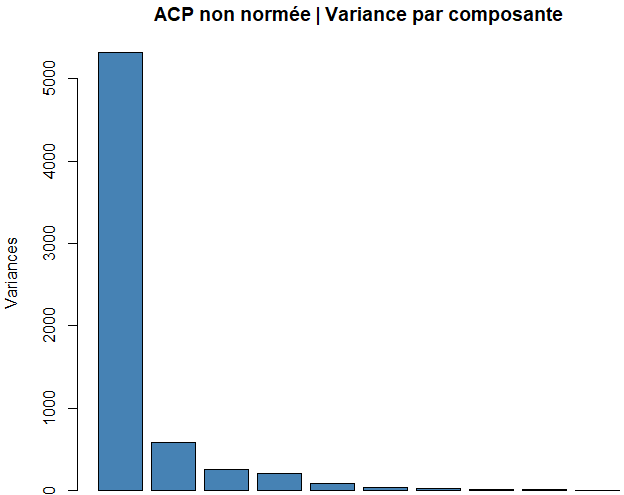
\includegraphics[width=\linewidth]{Image/fig_acp_brut_var.png}
    \caption{ACP non normée \phantom{x} | \phantom{x} variance par axe}
  \end{subfigure}
  \hfill
  \begin{subfigure}[b]{0.48\linewidth}
    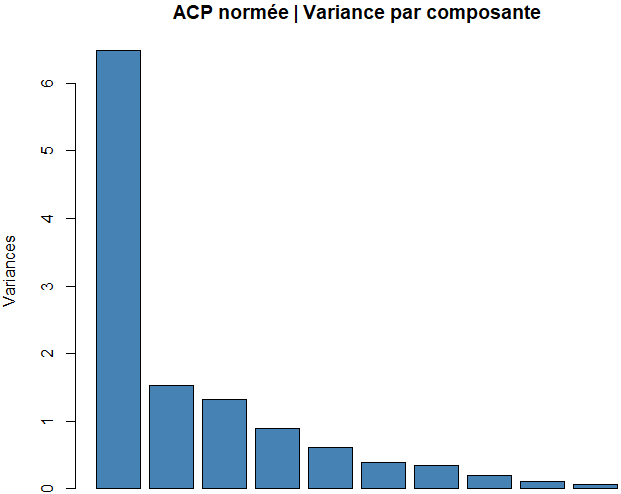
\includegraphics[width=\linewidth]{Image/fig_acp_norme_var.png}
    \caption{ACP normée \phantom{x} | \phantom{x} variance par axe}
  \end{subfigure}
  \caption{Éboulis des valeurs propres}
  \label{fig:acp_brut}
\end{figure}

\noindent L'\textbf{ACP normée} est retenue pour la suite. Chaque variable est
centrée-réduite avant l'analyse, garantissant une contribution équilibrée.

\subsection{Choix du nombre d'axes}

Les valeurs propres de l'ACP normée sont : $6.48$, $1.53$, $1.31$, $0.89$, $0.61$,\ldots
Selon la \textbf{règle de Kaiser} (valeurs propres $> 1$), \textbf{3 axes} sont
retenus. Ils expliquent cumulativement \textbf{77.7\,\%} de la variance totale
(PC1 : $54.0\,\%$, PC2 : $12.7\,\%$, PC3 : $11.0\,\%$).

\subsection{Interprétation des axes factoriels}

\begin{table}[H]
\centering
\caption{Loadings des variables sur les 3 premiers axes (ACP normée)}
\label{tab:loadings}
\small
\begin{tabular}{lrrr}
\toprule
\textbf{Variable} & \textbf{PC1} & \textbf{PC2} & \textbf{PC3} \\
\midrule
Batting\_average      & $-0.203$ & $-0.551$ & $\phantom{-}0.346$ \\
On\_base\_percentage  & $-0.228$ & $-0.465$ & $\phantom{-}0.409$ \\
Number\_of\_runs      & $-0.377$ & $-0.017$ & $-0.090$ \\
Number\_of\_hits      & $-0.370$ & $-0.030$ & $-0.076$ \\
Number\_of\_doubles   & $-0.344$ & $\phantom{-}0.046$ & $\phantom{-}0.025$ \\
Number\_of\_triples   & $-0.206$ & $-0.252$ & $-0.509$ \\
Number\_of\_home\_runs& $-0.296$ & $\phantom{-}0.373$ & $\phantom{-}0.254$ \\
Number\_of\_RBI       & $-0.356$ & $\phantom{-}0.225$ & $\phantom{-}0.140$ \\
Number\_of\_walks     & $-0.328$ & $\phantom{-}0.060$ & $\phantom{-}0.083$ \\
Number\_of\_strikeouts& $-0.298$ & $\phantom{-}0.364$ & $-0.080$ \\
Number\_of\_stolen\_bases & $-0.179$ & $-0.294$ & $-0.527$ \\
Number\_of\_errors    & $-0.153$ & $\phantom{-}0.038$ & $-0.253$ \\
\bottomrule
\end{tabular}
\end{table}

\begin{itemize}
  \item \textbf{PC1 (54\,\%) --- Axe de volume de jeu.} Tous les loadings sont
        négatifs : plus un joueur est à gauche sur cet axe, plus il a joué et
        produit (Hits, Runs, RBI, Doubles). C'est l'axe qui oppose les titulaires
        réguliers aux remplaçants.\vspace{0.3cm}
  \item \textbf{PC2 (12.7\,\%) --- Axe puissance vs précision.} Cet axe oppose
        les joueurs de puissance (HR et strikeouts élevés, valeurs positives) aux
        joueurs de contact (Batting\_avg et OBP élevés, valeurs négatives).\vspace{0.3cm}
  \item \textbf{PC3 (11.0\,\%) --- Axe vitesse vs puissance.} Cet axe oppose
        les joueurs rapides (triples, buts volés, valeurs négatives) aux frappeurs de
        puissance pure (HR).
\end{itemize}

\begin{figure}[H]
  \centering
  \begin{subfigure}[b]{0.40\linewidth}
    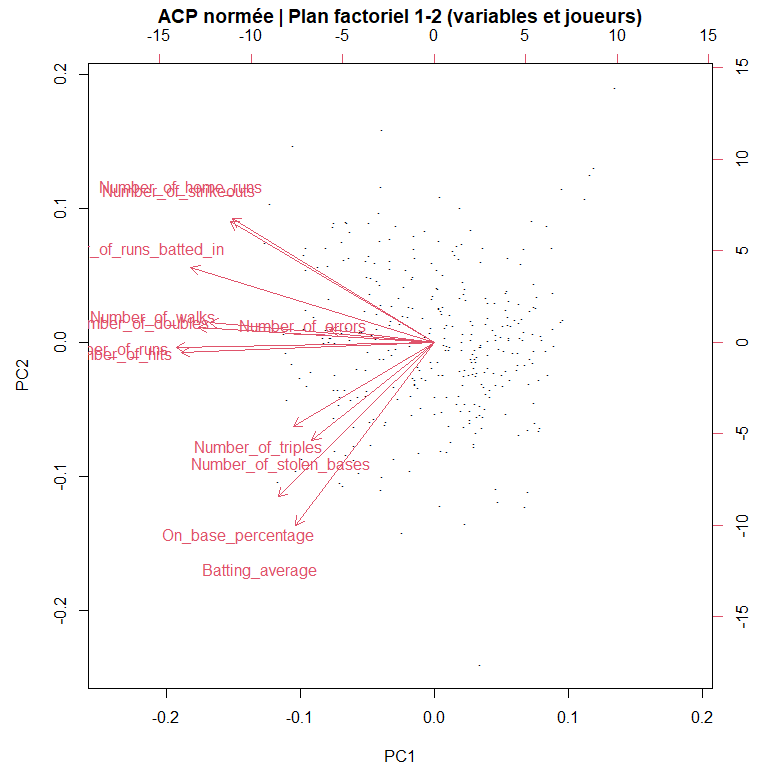
\includegraphics[width=\linewidth]{Image/fig_biplot_12.png}
    \caption{Plan factoriel 1-2}
  \end{subfigure}
  \hfill
  \begin{subfigure}[b]{0.40\linewidth}
    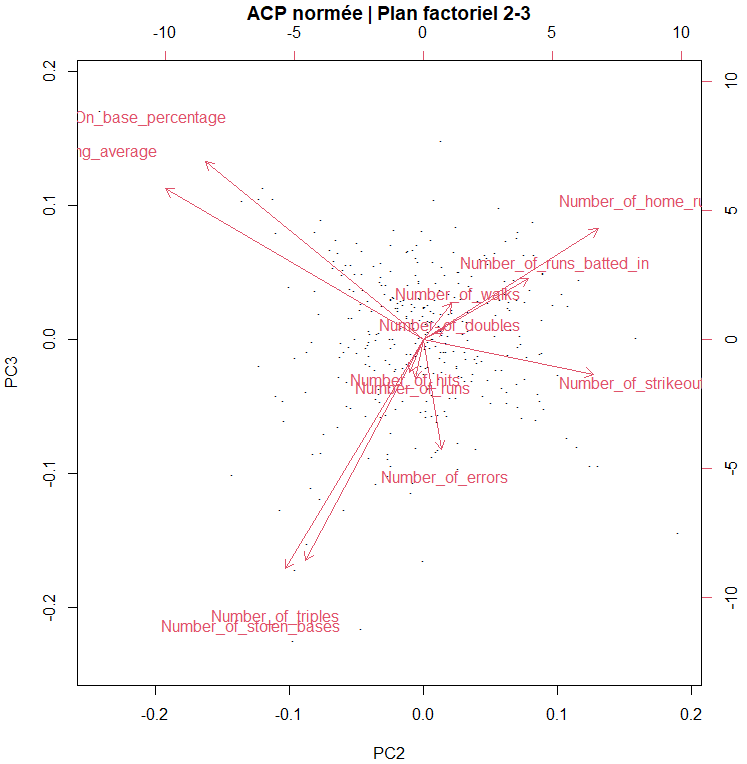
\includegraphics[width=\linewidth]{Image/fig_biplot_23.png}
    \caption{Plan factoriel 2-3}
  \end{subfigure}
  \caption{Biplots de l'ACP normée (variables en rouge, joueurs en gris)}
  \label{fig:biplots}
\end{figure}

\subsection{Classification Ascendante Hiérarchique}

\paragraph{Choix du nombre de clusters.}
Nous appliquons une CAH (méthode \textit{complete linkage}) sur les distances
euclidiennes calculées dans l'espace des 4 premières composantes principales.
Le critère du coude (figure~\ref{fig:coude}) indique un \textbf{saut maximal} entre
$k = 2$ (hauteur $\approx 14.2$) et $k = 3$ (hauteur $\approx 11.6$), suivi d'une
décroissance progressive. Nous retenons donc \textbf{$k = 3$ clusters}.

\begin{figure}[H]
  \centering
  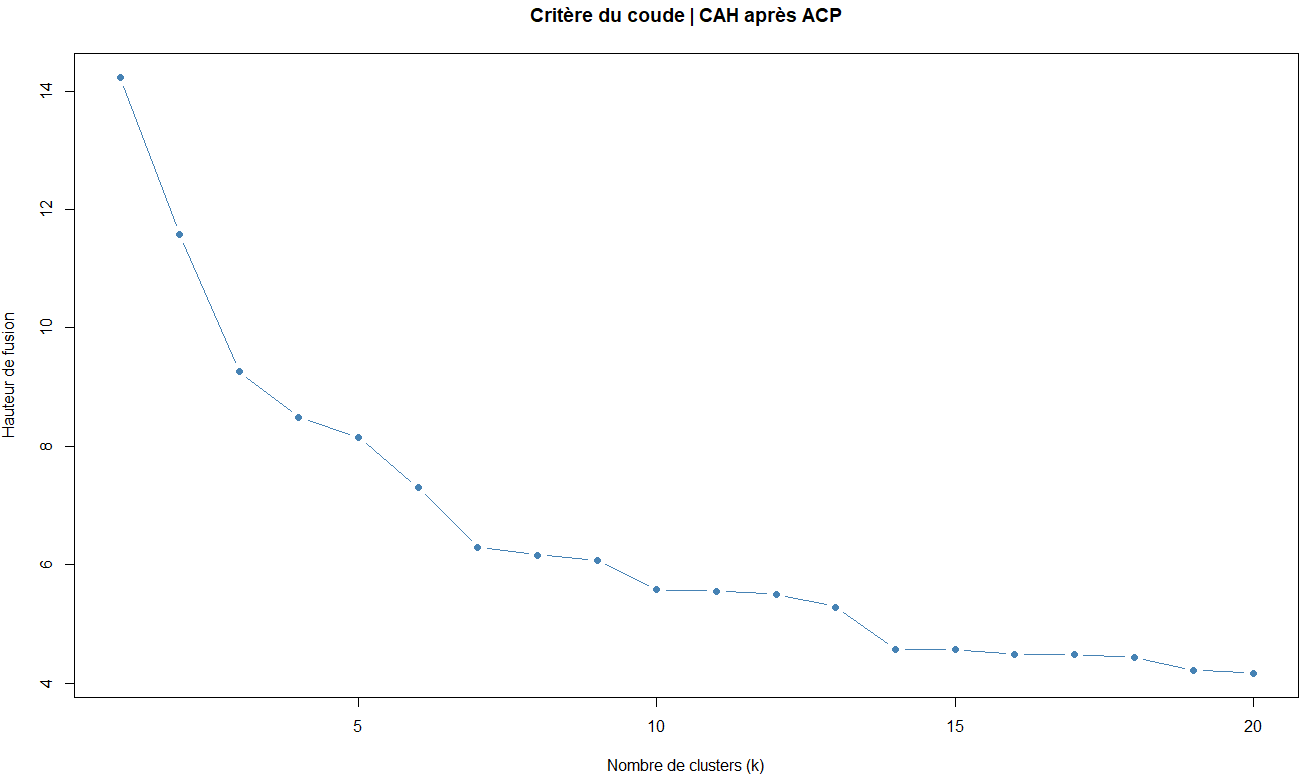
\includegraphics[width=0.9\linewidth]{Image/fig_coude.png}
  \caption{Critère du coude \phantom{x} | \phantom{x} CAH après ACP normée}
  \label{fig:coude}
\end{figure}

\paragraph{Profils des clusters.}

\begin{table}[H]
\centering
\caption{Profil moyen des 3 clusters}
\label{tab:clusters}
\small
\begin{tabular}{lrrr}
\toprule
\textbf{Statistique} & \textbf{Cluster 1} & \textbf{Cluster 2} & \textbf{Cluster 3} \\
  & \textbf{($n = 233$)} & \textbf{($n = 98$)} & \textbf{($n = 6$)} \\
\midrule
Batting\_average     & $0.267$ & $0.230$ & $0.356$ \\
On\_base\_percentage & $0.337$ & $0.288$ & $0.420$ \\
Hits                 & $117.7$ & $37.9$  & $23.0$  \\
Home\_runs           & $12.1$  & $2.5$   & $0.5$   \\
RBI                  & $56.7$  & $16.2$  & $7.5$   \\
Walks                & $44.9$  & $13.3$  & $7.3$   \\
Stolen\_Bases        & $10.8$  & $2.7$   & $0.5$   \\
\midrule
LogSalary moyen      & \textbf{6.943} & \textbf{5.663} & \textbf{4.947} \\
Salaire moyen        & $\approx 1\,040$~k\$ & $\approx 288$~k\$ & $\approx 141$~k\$ \\
\% free agency elig  & $48.1\,\%$ & $22.4\,\%$ & $0.0\,\%$ \\
\% arbitration elig  & $22.7\,\%$ & $12.2\,\%$ & $0.0\,\%$ \\
\bottomrule
\end{tabular}
\end{table}

Les trois groupes se distinguent clairement :
\begin{itemize}
  \item \textbf{Cluster 1 --- Titulaires réguliers (69\,\% des joueurs).}
        Ces joueurs présentent un fort volume de jeu (117 coups sûrs, 56 RBI en
        moyenne). Leur log-salaire moyen est le plus élevé ($6.94$) et ils sont les
        plus souvent éligibles à l'agence libre (48\,\%).\vspace{0.3cm}
  \item \textbf{Cluster 2 --- Remplaçants (29\,\% des joueurs).}
        Peu de coups sûrs (38), peu de RBI (16). Leur salaire est nettement plus
        bas (log-salaire $= 5.66$, soit $\approx 288$~k\$). Ce cluster correspond
        aux joueurs peu présents sur le terrain, sous contrat restreint.\vspace{0.3cm}
  \item \textbf{Cluster 3 --- Profils atypiques (6 joueurs).}
        Ces joueurs se distinguent par une excellente efficacité
        (\texttt{Batting\_avg} $= 0.356$, \texttt{OBP} $= 0.420$ --- valeurs exceptionnelles) mais
        un très faible volume de jeu (23 coups sûrs). Leur salaire est minimal
        (log-salaire $= 4.95$, $\approx 141$~k\$). Il s'agit probablement de
        jeunes joueurs très habiles mais peu exposés, ou de joueurs en sortie
        de blessure.
\end{itemize}

\begin{figure}[H]
  \centering
  \begin{subfigure}[b]{0.48\linewidth}
    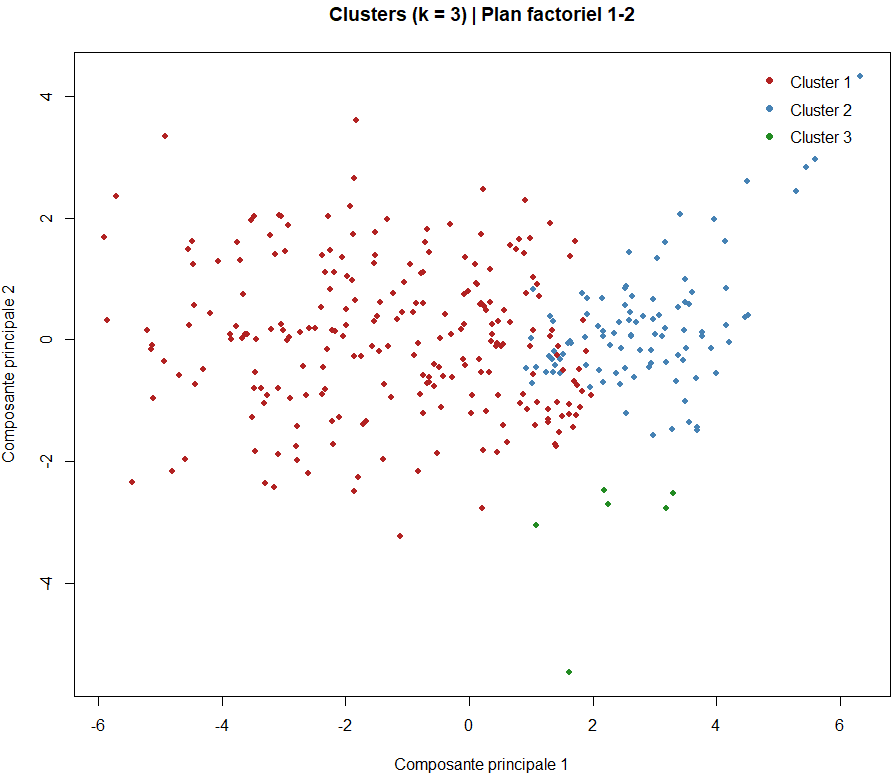
\includegraphics[width=\linewidth]{Image/fig_clusters.png}
    \caption{Clusters sur le plan factoriel 1-2}
  \end{subfigure}
  \hfill
  \begin{subfigure}[b]{0.48\linewidth}
    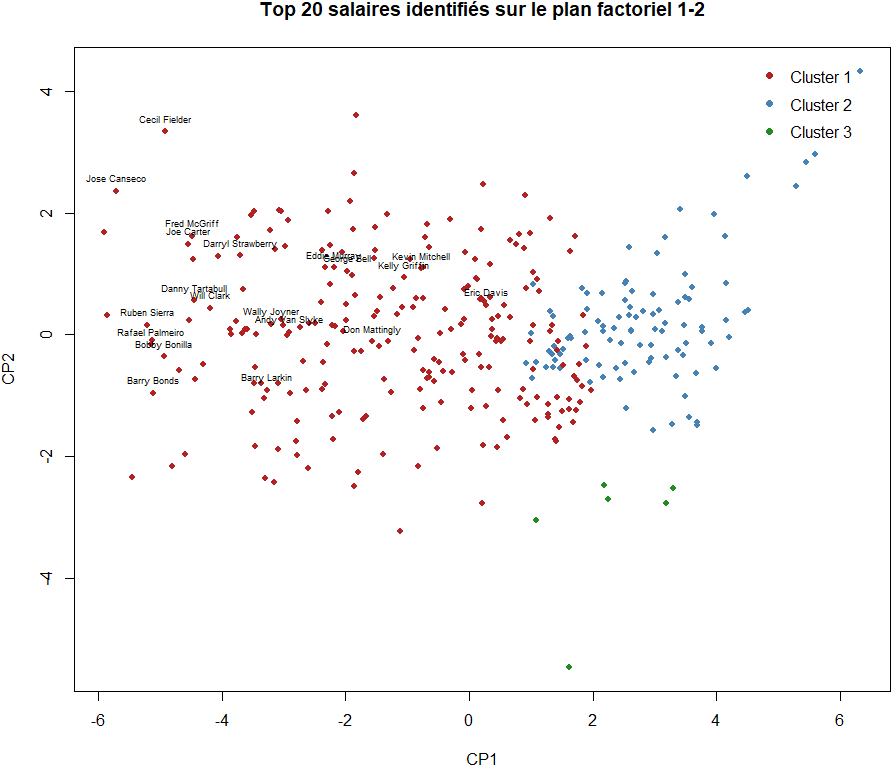
\includegraphics[width=\linewidth]{Image/fig_top20.png}
    \caption{Top 20 salaires identifiés}
  \end{subfigure}
  \caption{Visualisation des clusters dans l'espace factoriel}
  \label{fig:clusters}
\end{figure}

La figure~\ref{fig:clusters} (droite) confirme que les 20 salaires les plus
élevés (Bonds, Canseco, Fielder, McGriff\ldots) appartiennent tous au
\textbf{Cluster 1}, et se situent dans la partie gauche du plan factoriel, là
où les performances sont les plus élevées. Le volume de jeu est donc bien
la principale variable explicative du niveau de salaire.

% =============================================================================
\newpage
\section*{Conclusion}
\addcontentsline{toc}{section}{Conclusion}

Cette étude confirme que les salaires des joueurs de baseball en 1992 sont
\textbf{significativement déterminés par la performance}, mais que cette relation est
plus complexe que la simple équation «~meilleures stats = meilleur salaire~».\vspace{0.3cm}

Trois résultats principaux émergent. Premièrement, c'est le \textbf{volume de jeu} mesuré par le nombre de coups sûrs, de points marqués ou de RBI qui prédit
le mieux le salaire, davantage que des indicateurs de qualité pure comme la moyenne
au bâton. Deuxièmement, le \textbf{statut contractuel} joue un rôle prépondérant :
les agents libres perçoivent un salaire en moyenne quatre fois supérieur à celui des
joueurs sous contrat restreint, à performance égale. Cette prime reflète le pouvoir
de marché acquis avec la liberté de négociation. Troisièmement, l'ACP couplée à la
CAH révèle trois profils de joueurs bien distincts titulaires réguliers, remplaçants,
et profils atypiques efficaces mais peu utilisés dont les niveaux de salaire sont
parfaitement ordonnés.\vspace{0.3cm}

Ces résultats sont cohérents avec la littérature en économie du sport et permettent de mieux comprendre pourquoi l’Association des joueurs a obtenu gain de cause dans le litige concernant la sous-rémunération des agents libres en 1991/92 : la régression multiple met en évidence un coefficient négatif pour les agents libres récents, ce qui suggère l’existence d’une entente implicite entre clubs.\vspace{0.3cm}

Pour de futurs travaux, il serait pertinent d’intégrer des données couvrant plusieurs saisons consécutives afin d’étudier l’évolution des salaires, ou encore d’utiliser des méthodes non linéaires (forêts aléatoires, boosting) pour améliorer les performances prédictives du modèle.\vspace{1cm}

% =============================================================================
\begin{thebibliography}{9}

\bibitem{watnik1998}
Watnik, M.~R. (1998).
\textit{Pay for Play: Are Baseball Salaries Based on Performance?}
Journal of Statistics Education, 6(2).\vspace{0.3cm}

\bibitem{neter1996}
Neter, J., Kutner, M.~H., Nachtsheim, C.~J., \& Wasserman, W. (1996).
\textit{Applied Linear Statistical Models} (4th ed.).
Chicago: Irwin.\vspace{0.3cm}

\bibitem{christensen1996}
Christensen, R. (1996).
\textit{Analysis of Variance, Design and Regression}.
London: Chapman and Hall.

\end{thebibliography}

\end{document}